\documentclass[twocolumn]{article}
\usepackage{graphicx}
\usepackage{amsmath}
\usepackage{amssymb}
\usepackage{subfigure}
\usepackage{epstopdf}
\usepackage{setspace}
\onehalfspacing
\epstopdfsetup{update} % only regenerate pdf files when eps file is newer
\title{Tuning plasmon of gold nanorods by KCN etching}
\author{Aquiles Carattino \and Saumya Khatua \and Michel
Orrit}

\begin{document}
\maketitle
\abstract{This is the abstract}

\section{Introduction}
In recent years gold nanoparticles received a great amount of attention because
of their size-dependent optical properties \cite{Zijlstra2011}. Gold
nanoparticles have shown to be suitable for a range of experiments and
applications extending from solar cells production \cite{Catchpole2008} to
biosensing \cite{Zijlstra2012}, photodynamic therapy \cite{Zhao2014},
plasmon-enhanced spectroscopies \cite{Sivapalan2013}, bioimaging
\cite{VandenBroek2013}, etc. and they can also be used as building blocks for
bigger nanostructures \cite{Ivanov2011} \cite{Do2013} \cite{Guffey2011}. These
versatility is mainly given by the presence of a collective oscillation of
conduction electrons known as surface plasmon; for the case of gold nanorods
(AuNR) its resonance energy (SPR) depends on the aspect ratio (AR) of the
particle and can be found between $2.3\,\textrm{eV}$ for spheres (AR of $1$) to
even below $0.8\,\textrm{eV}$ for very elongated particles (i.e. they can cover
almost the entire visible spectrum and near infrared.)

Controlling the resonance of the particles is useful when is needed to have
control over the spectral properties of these structures. In almost all the
applications cited above, the SPR is critical for a successful experiment.
Moreover, it may just be needed to have a particle with a resonance coinciding
with the available lasers; or the control over the spectral response of the
particles can be used for generating narrow transparency windows
\cite{Biswas2013}. It was also shown, for instance, that Surface Enhanced Raman
Spectroscopy (SERS) depends highly the plasmon resonance of the particles
employed \cite{Sivapalan2013}. In any case this is only a short list to
highlight the importance of the position of the SPR peak.

One of characteristic that makes gold nanorods versatile is the easiness with
which the resonance peak can be tuned. Usually this is done at the moment of
synthesis \cite{Gou2005}, by controlling the concentrations of growth and seed
solutions it is possible to induce the formation of longer or shorter particles
\cite{Nikoobakht2003}. This methods, however, always present a dispersion in the
size distribution of the outcome, hindering the repeatability and the ability to
build larger, periodic structures.

It is therefore useful a method that allows the in-\textit{situ} control of the
plasmon resonance. This work shows that is possible to change the plasmon
resonance peak in more than $300\,\textrm{meV}$ without degrading the optical
properties (i.e. the FWHM of the peak.) For doing so it is employed KCN as an
etching agent; a known and well understood compound that is used not only in the
nano-industry but also at bigger scales, for instance for gold mining. It's
overall reaction formula is:
\begin{equation*}
4\textrm{Au} + 8\textrm{KCN}^-+\textrm{O}_2 + 2\textrm{H}_2\textrm{O}
\leftrightarrows 4K\textrm{Au(CN)}_2^-+4\textrm{KOH}^-
\end{equation*}
In bulk this compound was used for reducing the aspect ratio of rods, i.e.
blue shifting their plasmon \cite{Jana2002}. In a more recent paper it was also
used for generating highly spherical particles with a narrow size
distribution \cite{Lee2013}.

In this work the opposite trend is observed. Single-particle experiments of the
AuNR immersed in KCN show a red-shift of the plasmon meaning an increase in
their aspect ratio. This is confirmed by tracking the luminescence spectra of
individual rods over time as well as by acquiring SEM images of them. A simple
model where etching is considered as being isotropic and constant (i.e. both the
radius of the particle and it's length diminish at the same rate over time),
yields a good agreement with both sets of experiments.

\section{Experimental method}
The luminescence spectra of single gold nanorods (AuNR) is acquired in a home
built confocal microscope using an Acton 500i Spectrometer. A $532\,\textrm{nm}$
laser is used for exciting the particles with a power in the back focal plane of
of the objective of $300\,\mu\textrm{W}$. A high NA objective (Olympus $60$X NA
$1.4$ Oil immersion) is used for both focusing the laser and collecting the
luminescence. A $532\,\textrm{nm}$ notch filter cuts out the excitation light.

The samples are prepared by spin casting a suspension of AuNR on clean
coverslips and thoroughly rinsing them  with Milli-Q water for eliminating the
excess of CTAB. The samples are then placed in a flowcell; the initial spectra
are taken with the rods immersed in Milli-Q water. This characterization allows
to discard, for instance, clusters of rods. After this, a solution of KCN is
flowed into the cell with concentrations ranging from $3\mu\textrm{M}$ to
$50\mu\textrm{M}$. Then the spectra of approximately $10$ different particles is
acquired consecutively after focusing in each one. The time resolution varies
according to the exposure time and number of particles; in this work a spectra
is taken at least every minute.

For confirming the shape of the particles after the dissolution in KCN, SEM
images are acquired. The samples are prepared by letting a droplet of a
suspension of AuNR dry on top of a silicon wafer and then thoroughly rinsing
them with Milli-Q water for eliminating the excess of CTAB. The same samples are
employed for taking images before and after immersing the particles in
$30\mu\textrm{M}$ KCN. For the analysis only the rods separated from each other
are considered as to reproduce the conditions found in the optical experiment.
After immersing the samples in KCN for a given period of time, they are rinsed
with water to stop the reaction and dried with a nitrogen flow.

Bulk extinction spectra of the suspension of rods used previously is acquired as
a function of time after a solution of KCN is added into the vial. This allows
to compare single-particle experiments with previous results. 

\section{Results and discussion}

Figure \ref{fig:plasmon_single_rod} shows the typical behavior of the plasmon of
a single rod while immersed in $30\,\mu\textrm{M}$ KCN; it can be seen the
luminescence spectra in intervals of $70\,s$ between each other; the small
shoulder at $1.9\,\textrm{eV}$ ($650\,\textrm{nm}$) that can be observed for the
less intense curves is due to Raman scattering of water that was not completely
removed when subtracting the background to these curves. The inset shows the
peak position (calculated by fitting the spectra with a lorentzian) over time.
It can be seen that the plasmon red-shifts over $0.25\,\textrm{eV}$
($100\,\textrm{nm}$) in $5$ minutes. It is possible to observe that the optical
properties of the plasmon do not get dampered by studying the FWHM of the peak.

Figure \ref{fig:FWHM} shows the FWHM of the plasmon as a function of plasmon
shift for a collection of nanorods immersed in KCN. At first there is a
rapid diminishing of the width, reaching a minumum for shifts between
$0.15\,\textrm{eV}$ and $0.20\,\textrm{eV}$. The rapid decrease in width is
probably due to the elimination of impurities on the surface of the
particles, since they tend to be more reactive. The following narrowing merits
an electronic explanation; the higher energy distance between the longitudinal
plasmon peak and interband transitions in gold makes less efficient the damping
mechanisms in the particles, hence yielding a narrower resonance. While the
reaction continues, the width starts to increase; this means that the reshaping
at some point will start having an effect on the shape of the particle. This is
often encountered for shifts above $0.15\,textrm{eV}$, but depends on the
particle initial size and shape. ADDA simulations allow to confirm that
the reshaping of the particles induces a width change. 

The inset in Figure \red{fig:FWHM} shows the results of the ADDA simulations
for a $25x60$nm particle while both its axis diminish evenly. The initial width
is $0.14\,textrm{eV}$, that is normally lower than the experimentally
obtainable. This is due to particles not having a perfect rod shape, or defects
in their crystalline structure. The calculated width however diminishes to
$0.1\,\texrm{eV}$ for shifts of just under $0.2\,\textrm{eV}$ as it is observed
experimentally. This is already showing an agreement between a model of
isotropic etching and our experimental results, and can also be compared to the
plasmon peak shift of different particles. 

Figure \ref{fig:plasmon_average} shows the time traces of the peak positions for
nine different rods while being etched with $30\,\mu\textrm{M}$ KCN. The pale
lines show each individual trace, while the darker is the average.
The error bars are the standard deviation of the distribution at each point.
Since spectra of different particles are taken at slightly different times (one
after the other), an interpolation with cubic splines is used for calculating
the average and the standard deviation at the given times. The bigger time step
between $225\,\textrm{s}$ and $340\,\textrm{s}$ is due to an automatic
refocusing happening on the particles every $5$ minutes.

The diminishing intensity is consistent
with the volume loss given by the dissolution of gold.
In this particular case only one rod is observed therefore having a higher
temporal resolution. However the same trend is followed by each single nanorod
analyzed under the same conditions.


\begin{figure}[tp]
 \centering
 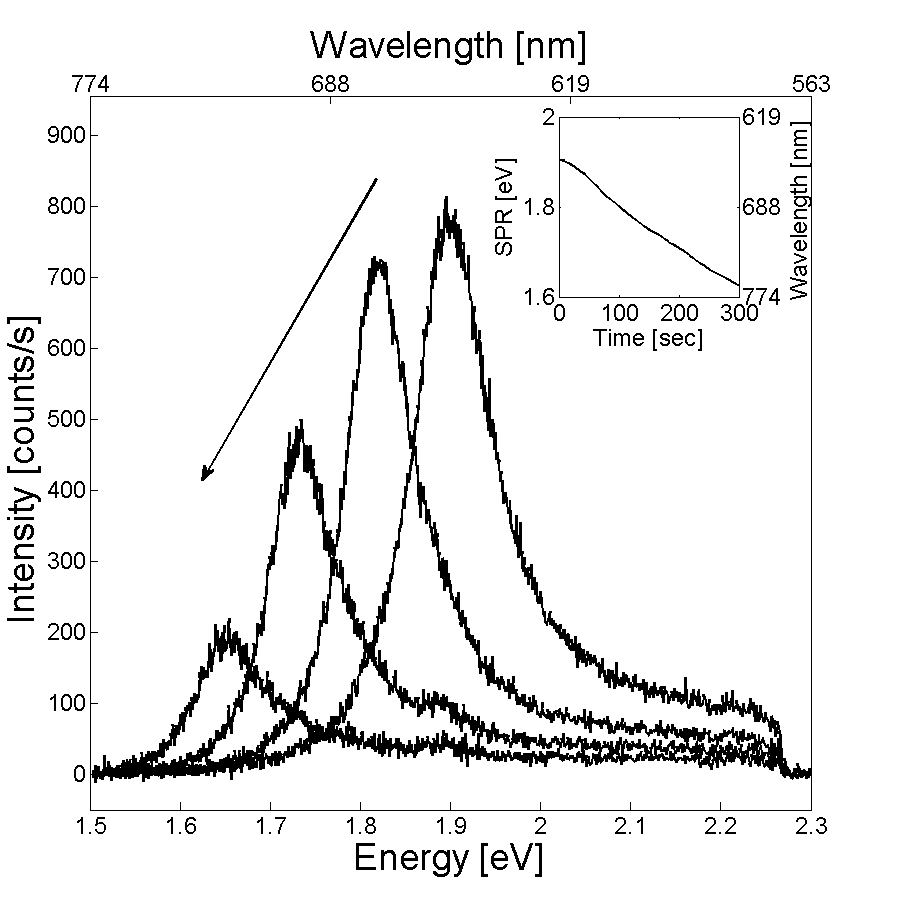
\includegraphics[width=0.95\linewidth]{plasmon_single_rod.png}
 \caption{Plasmon shift due to the etching with $30\mu M$ KCN. The time
 interval between peaks is $70s$. The inset shows the peak position of the SPR as a
 function of time, extracted by fitting the spectra with a lorenzian.}
 \label{fig:plasmon_single_rod}
\end{figure}

These results show the opposite trend than the bulk results and therefore need a
closer study. F

\begin{figure}[tp]
 \centering
 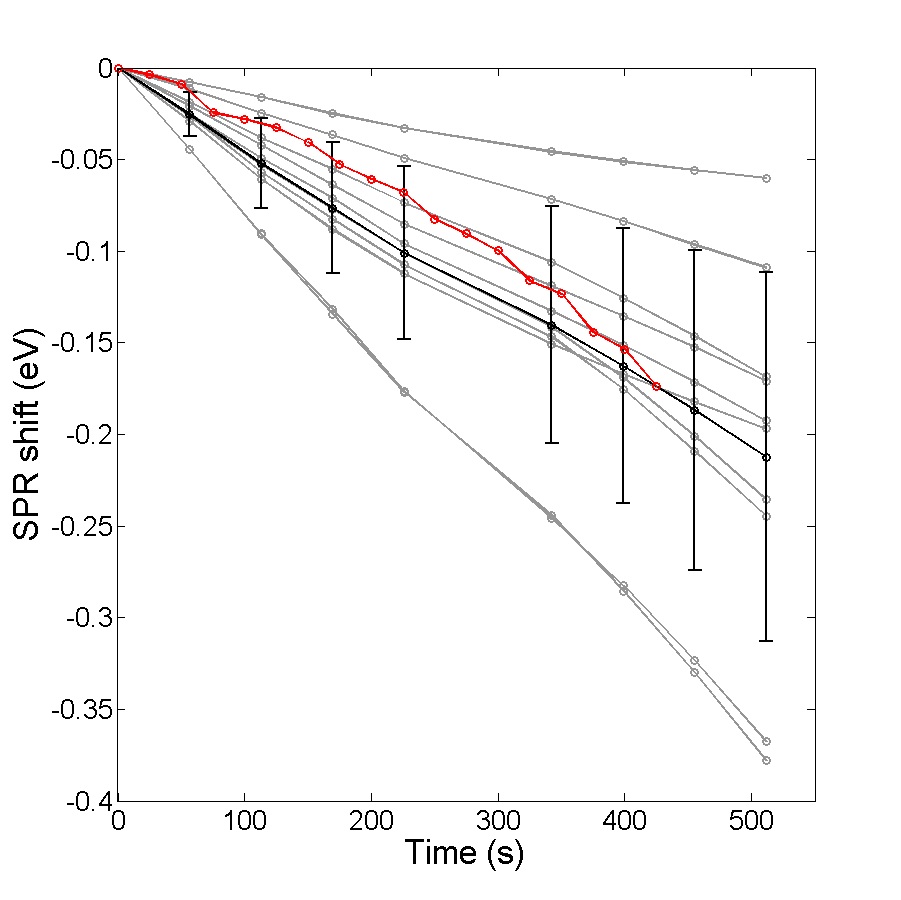
\includegraphics[width=0.95\linewidth]{plasmon_average.png}
 \caption{Average plasmon shift (thick line) for 9 rods due to the etching with
 $30\mu M$ KCN. The light curves are individual time traces while the thick one
 is the average. The error bars are simply the standard deviation at each point. Over
 time the peak distribution gets broader.}
 \label{fig:plasmon_average}
\end{figure}

This exact same trend is observed for every particle at different KCN
concentrations. The broadening of the distribution is also observed and has to
be attributed to intrinsic inhomogeneities in the particles since it is not
possible to find a trend in the shift rate nor with the initial particle 
volume nor with the initial peak position. 
% How can this be explained????

One important aspect of these results is that despite the broadening in plasmon
peak distribution over a sample the width of the plasmon peak of each individual
rod does not increase. 

\begin{figure}[tp]
 \centering
 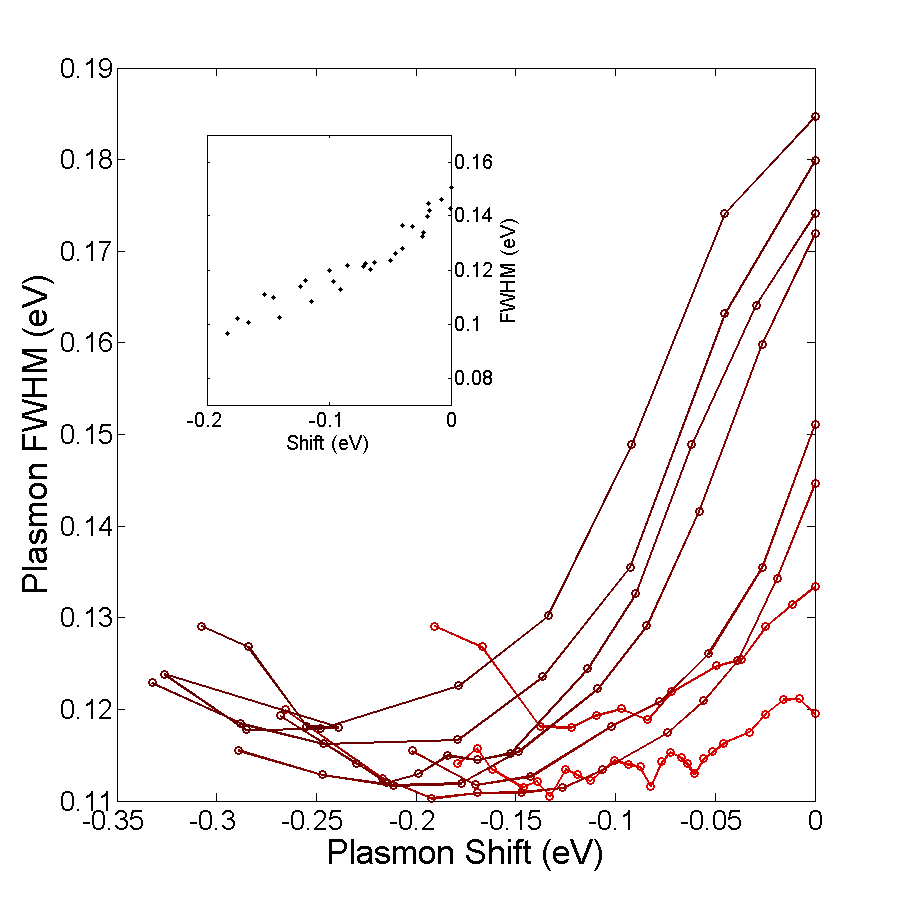
\includegraphics[width=0.95\linewidth]{fwhm_several_in_eV.png}
 \caption{Plasmon FWHM of eight different particles immersed in $30\,\mu M$ KCN
 as a function of their plasmon shift. The inset shows the results from the
 simulations carried on with the ADDA package.}
 \label{fig:FWHM}
\end{figure}

For understanding these results a simple model of isotropic etching may be
considered. It is assumed that the nanorods diminish their length and radius at
the same rate. The extinction cross section spectra is then calculated for
several time steps using the ADDA package \cite{Yurkin2011}. The peaks are
extracted from the simulations in the same way than for the experiments. The
results are displayed as the red curve in Figure \ref{fig:plasmon_average}. The
best approximation to the average is found when the etching rate is set to
$1\,\textrm{nm}/min$.

The optical properties of the single-particles were correlated with SEM images
(see supporting information) of samples of the same nanorods before the etching,
after $2\,\textrm{min}$ submersed in KCN and after $4\,\textrm{min}$. The main
important observation is the preservation of the shape. When particles are
isolated from each other, the model of the isotropic etching seems appropriate.
Calculating the distribution of sizes of the particles show a slight increase in
the aspect ratio but this is however obscured by the broad distribution of
values (even before starting the etching). Averaging around $300$ different
particles at each interval yields an etching constant of
$0.5\,\textrm{nm}/\min$, consistent with the optical observations.

As stated previously, the first experiment performed is the bulk measurement in
a UV-VIS spectrometer. The extinction spectra of the suspension of rods as a
function of time can be seen in Figure \ref{fig:bulk}. The main plot shows the
spectra at intervals of of $9$ minutes after adding a solution of KCN. This
solution is chosen as to have $50\mu\textrm{M}$ KCN in the vial where the
suspension of AuNR is present. Since after the first $9$ minutes there is no appreciable
change in the peak position, the same amount of KCN is added into the vial,
yielding a concentration of $100\,\mu\textrm{M}$. This explains the sudden
change in the time-trace depicted in the inset of the Figure. All spectra plots are
normalized to the transverse plasmon peak at $2.4\,\textrm{eV}$ for increasing
the visibility of the plasmon shift.

\begin{figure}[tp]
 \centering 
 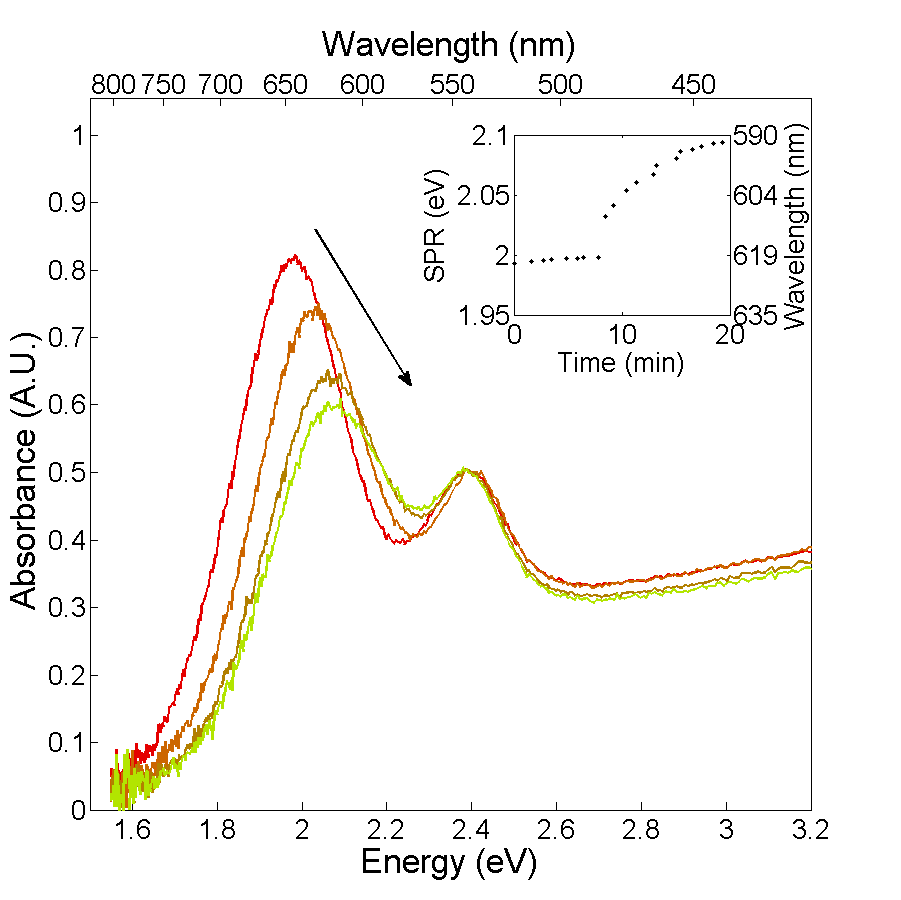
\includegraphics[width=0.95\linewidth]{plasmon_bulk.png}
 \caption{Bulk extinction spectra at $10$ minutes time-interval. The arrow
 indicates the time evolution. A solution of KCN is added into the cuvette with
 the nanorod suspension as to have a $50\,\mu M$ concentration for the first 9
 minutes; then this step is repeated, yielding a final KCN concentration of
 $100\, \mu M$. The inset shows the peak position of the SPR position as a
 function of time, extracted by fitting the spectra with a lorentzian.  }
 \label{fig:bulk}
\end{figure}

It can be seen that the plasmon peak position shifts towards higher energies
(from approximately $2.0\,\textrm{eV}$ to $2.1\,\textrm{eV}$ or equivalently
from $620\,\textrm{nm}$ to $592\,\textrm{nm}$). It means that the rods are
reshaping into spheres as was previously observed \cite{Jana2002}. The
asymptotic behavior of the time-trace may be due to the small amount of KCN
added into the vial, that reacts entirely with gold therefore stopping the
effect after a certain time.

\section{Conclusions}
In this work we have shown a simple method that allows the tuning of the plasmon
peak position of single gold nanorods with nanometer accuracy. More
importantly, it is shown that the rodlike shape is preserved even for plasmon
shifts of approximately $300\,\textrm{meV}$ ($80\,\textrm{nm}$) therefore
keeping the well known properties of them.

The optical experiments show the shift of the plasmon with a high time accuracy,
allowing to stop the reaction when the peak is at the desired value. SEM images
allow to confirm that the shape of the rods is being preserved.The agreement
between the simulations and the experimental results not only show the link
between both measurements but also provide a way of predicting the behaviour of
the plasmon peak.

However, it is also found a great distribution width of the rate at which the
plasmon peak shifts for different particles under the same experimental
conditions. This can be explained only considering that there is an intrinsic
difference between particles; this differences can be attributed to defects on
the particle surface or to inhomogeneities in the left over CTAB capping the
rods even if care is taken to remove it by rinsing with water. Different initial
conditions (such as initial aspect ratio or volume) were considered but no
correlation with the rate of the shift is observed.

Combining this results with the catalytic properties of gold and the presence of
the plasmon resonance opens the door for fine-controlling chemical reactions
while irradiating the particles with specific wavelengths. On the other hand
this same technique can be used for detecting the presence of KCN in a
solution. This result was already reported by Wei et Al. in 2012 \cite{Wei2012}
in a slightly different condition. We believe that the sensitivity of single
particles to very low concentrations (in the order or below the pM) should be
higher.

\bibliography{bibliography}{}
\bibliographystyle{ieeetr}

\end{document}
